\documentclass[svgnames]{beamer}

% https://iccl.inf.tu-dresden.de/w/images/d/d3/Lecture-07.pdf

\usepackage[utf8]{inputenc}
\usepackage[english,russian]{babel}
\usepackage{cmap}
\hypersetup{unicode=true}
\graphicspath{{images/}{slides/images}}

\title[CMTA 06]
{Distributional Semantics}
\subtitle
{Computational Methods for Text Analysis}
\author
{Alena Pestova}
\institute
{HSE Saint-Petersburg}
\date
{08.11.2022}

\subject{natural language processing, text mining}


\newcommand{\tb}[1]{\colorbox{yellow}{#1}\space}
\newcommand{\Sp}[1]{\colorbox{green}{#1}\space}
\newcommand{\Sn}[1]{\colorbox{red}{#1}\space}


\begin{document}

    \begin{frame}
        \titlepage
    \end{frame}


    \begin{frame}
        \frametitle{The Distributional Hypothesis}
        \begin{block}{Firth 1957}
            You shall know a word by the company it keeps.
        \end{block}

    \end{frame}

    \begin{frame}
        \frametitle{The Distributional Hypothesis}

        \begin{block}{Harris 1954}
            The fact that, for example, \alert{not every adjectives occurs with every noun} can be used as
            a \alert{measure of meaning difference}. For it is not merely that different members of the
            one class have different selections of members of the other class with which they are
            actually found. More than that: if we consider words or morphemes A and B to
            be more different than A and C, then we will often find that the distributions of A and
            B are more different than the distributions of A and C. In other words, \alert{difference in
            meaning correlates with difference in distribution}.
        \end{block}

        In simple words: words that occur in the same contexts tend to have similar meanings.
    \end{frame}


    \begin{frame}{Example}
        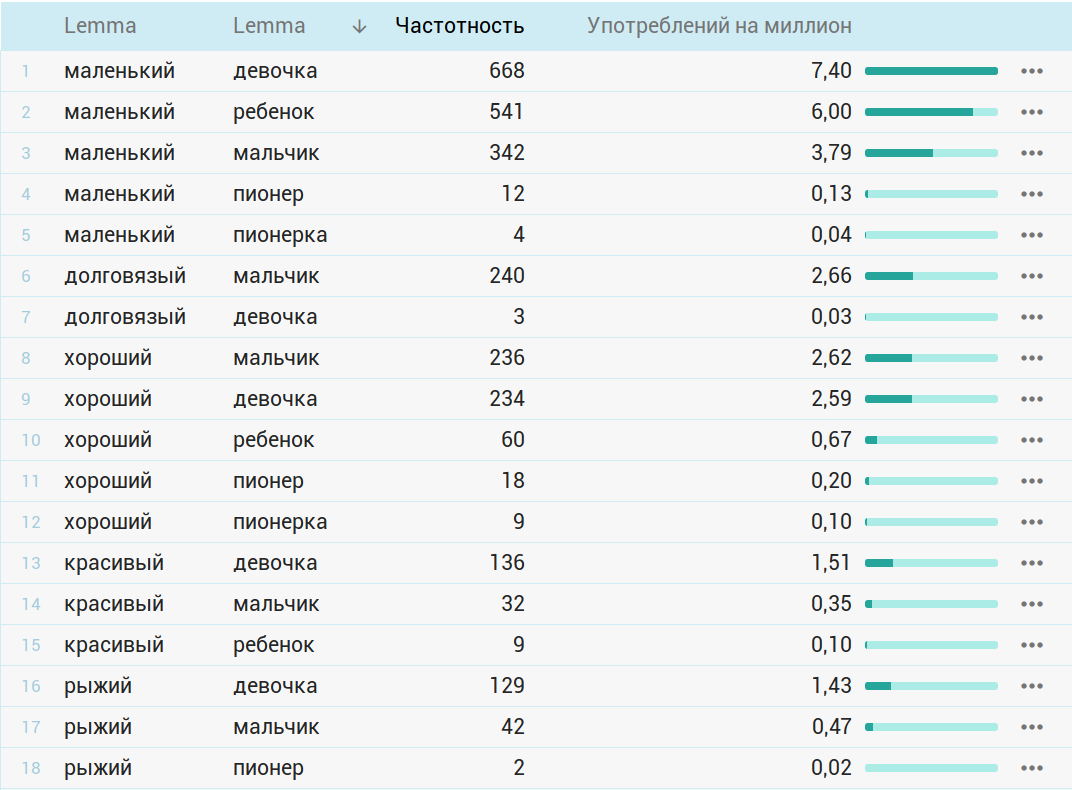
\includegraphics[width=.9\textwidth]{adjectives.png}
    \end{frame}


    \begin{frame}{Why is it useful?}
        \begin{itemize}
            \item we can try to use this knowledge for building word vector representations
            \item they will help us to solve very different tasks
        \end{itemize}
    \end{frame}


    \begin{frame}{Distributional Semantic Models}
        \begin{itemize}
            \item words are represented as real-valued vectors built from their
            distribution in contexts
            \item similarity between words is approximated in terms of their
            geometric distance between vectors
            \item build as general-purpose semantic models that can be applied
            to various tasks (resulting vectors are not task specific)
            \item rely on a co-occurrence matrix
        \end{itemize}
    \end{frame}


    \begin{frame}{Co-occurence matrix}
        \begin{itemize}
            \item Each row in the matrix $M$ represents a word $w_i$
            \item Each column in the matrix $M$ represents a context $c_j$
            (depending on window size: number of words in the context
            considered; frequently paragraphs or documents as below)
            \item Matrix $M_{ij}$ represents the strength of association
            \item term-document matrices can get very large => need dimensionality
            reduction
            \item compute similarity between two words based on row vectors
        \end{itemize}
        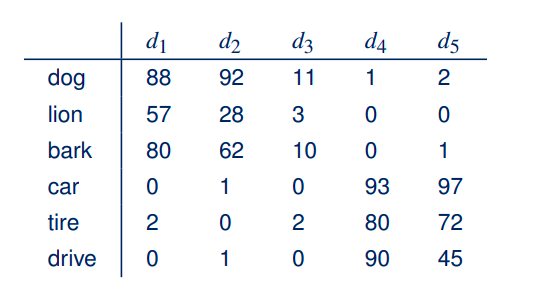
\includegraphics[width=.6\textwidth]{co-occurence-docs.png}
    \end{frame}

    \begin{frame}{Association and similarity}
        \begin{itemize}
            \item Pointwise-mutual information (PMI)
            \item Cosine similarity/distance between vectors
        \end{itemize}
    \end{frame}

%    \begin{frame}{Co-occurence matrix}
%        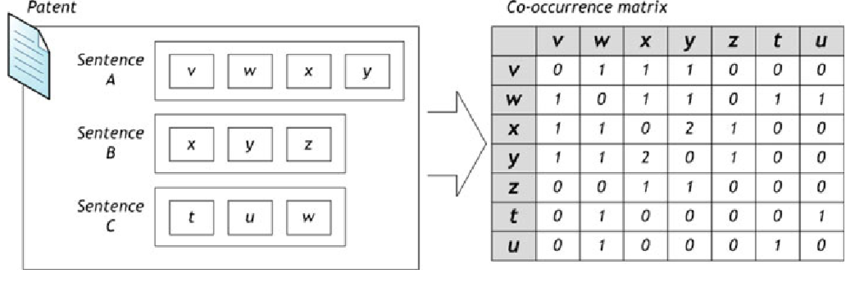
\includegraphics[width=.9\textwidth]{co-occurence.png}
%    \end{frame}


    \begin{frame}{Dimensionality Reduction}

        One available method is Singular Value Decomposition (SVD)):
        \begin{itemize}
            \item Factorizes matrix M into three matrices: $M_{m,n} = U_{m, m} \Sigma_{m, n} V_{n, n}^T$
            \item $U$ and $V$ represent orthogonal matrices and $\Sigma$ is a diagonal matrix
            \item we want to select the k top singular values to obtain lower
            dimensional vectors that account for the maximum proportion
            of the original variance
            \item we want to get the best rank-d approximation of $M$
            \item computing the truncated projection: $M_{reduced} = U_{m, k} \Sigma_{k, k}V_{n, k}^T$
            \item now, we have vectors with length less than original vectors
        \end{itemize}
    \end{frame}

    \begin{frame}
        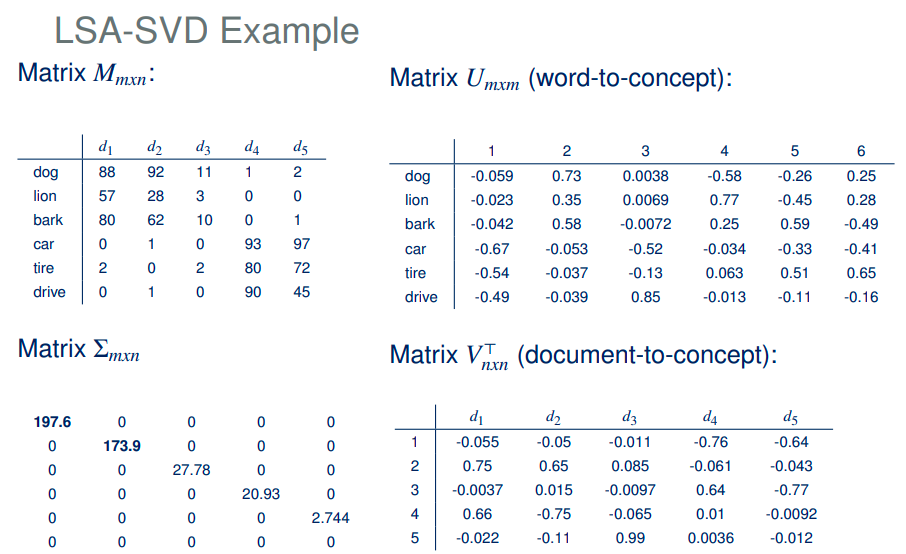
\includegraphics[width=.9\textwidth]{lsa-svd1}
    \end{frame}

    \begin{frame}
        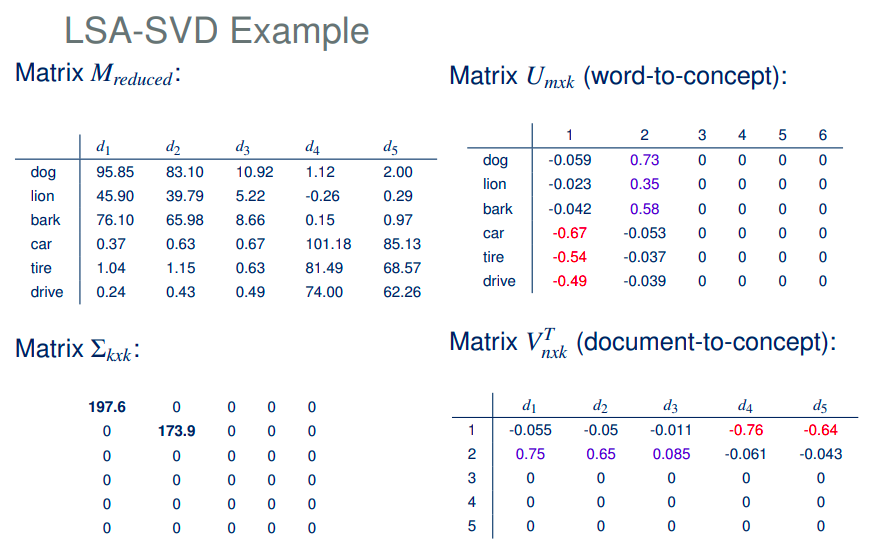
\includegraphics[width=.9\textwidth]{lsa-svd2}
    \end{frame}

    \begin{frame}{LSA-SVD Example}
        \begin{itemize}
            \item Cosine similarity between d1 and d3 originally ≈ 0.96
            \item Cosine similarity between d1 and d3 reduced ≈ 0.99
            \item Cosine similarity between lion and car originally ≈ 0.0033
            \item Cosine similarity between lion and car reduced ≈ 0.0054
            \item etc.
        \end{itemize}
    \end{frame}

    \begin{frame}{Latent Semantic Analysis (LSA)}
        Words and documents - vectors in the semantic space, dimensions
        which are "latent" variables.
        \begin{itemize}
            \item co-occurring words are projected onto the same dimensions;
            \item vector for the document - the weighted sum of the vectors of the words included in it (centroid);
            \item in semantic space the angle between document vectors
            may be small, \alert{even if there are no common words in the documents}.
        \end{itemize}
    \end{frame}

%\begin{frame}{LSA}
%        Evaluation of  semantic proximity (similarity):
%        \begin{itemize}
%            \item word—word
%            \item word—document
%            \item document—document
%            \item document-word
%        \end{itemize}
%        Typical applications of LSA:
%        \begin{itemize}
%            \item search for documents close to the query (killer feature for
%            information search);
%            \item detection of semantically close words (synonyms);
%            \item evaluation of text coherence (semantic similarity of neighboring paragraphs);
%            \item extract keywords of the text.
%        \end{itemize}
%    \end{frame}
%\end{document}


    \begin{frame}{Disadvantages of LSA-SVD}
        \begin{itemize}
            \item Relatively poor quality of obtained representstions
            \item The complexity of working with a very large and sparse matrix
            \item Difficulty in adding new words/documents
        \end{itemize}
    \end{frame}


    \begin{frame}{Word Embeddings}

        Definition: Real-valued and sub-symbolic representations of words as dense
        numeric vectors.

        \begin{itemize}
            \item distributed representation of word meanings (not
            count-based)
            \item usually learned with neural networks
            \item specific dimensions of the resulting vectors cannot bet directly
            mapped to symbolic representation
            \item models that seek to predict between a center word and
            context words (predict models)
            \item key elements of deep learning models
        \end{itemize}
    \end{frame}

    \begin{frame}{Word Embeddings}
        Word Embeddings (WE) is a popular framework in NLP that allows to represent meaning of words and phrases as vectors of real numbers (Mikolov et al., 2013).

        WE has become a very common in many NLP tasks, such as machine translation, classification, document ranking, sentiment analysis.
    \end{frame}

    \begin{frame}{Methods to Train Word Embeddings}
        \begin{itemize}
            \item word2vec (CBOW and SGNS)
            \item FastText - extension of Word2Vec, train on subword information (n-grams)
            \item Clove
            \item and many others (with almost all other NLP neural networks)
        \end{itemize}
    \end{frame}

    \begin{frame}{Idea of word2vec}
        Framework for learning word embeddings; main idea:
        \begin{itemize}
            \item takes words from a very large corpus of text as input
            (unsupervised)
            \item learn a vector representation for each word to predict between
            every word and its context
        \end{itemize}

        Two main algorithms:

        \begin{itemize}
            \item Continuous Bag of Words (CBOW): predicts center
            word from the given context (sum of surrounding words
            vectors)
            \item Skip-gram (SGNS): predicts context taking the center word as
            input
        \end{itemize}
    \end{frame}


    \begin{frame}{Idea of word2vec}
        Don’t count, predict!
        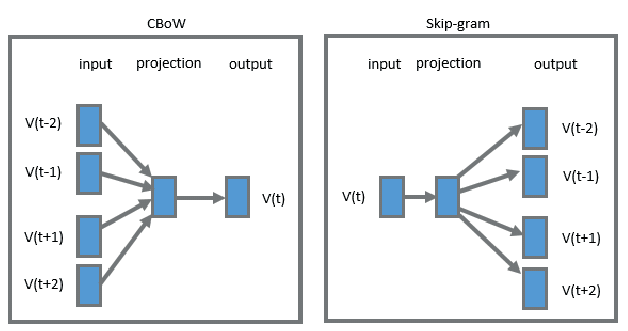
\includegraphics[width=\textwidth]{cbow_sgns}
    \end{frame}

    \begin{frame}{Idea of word2vec}
        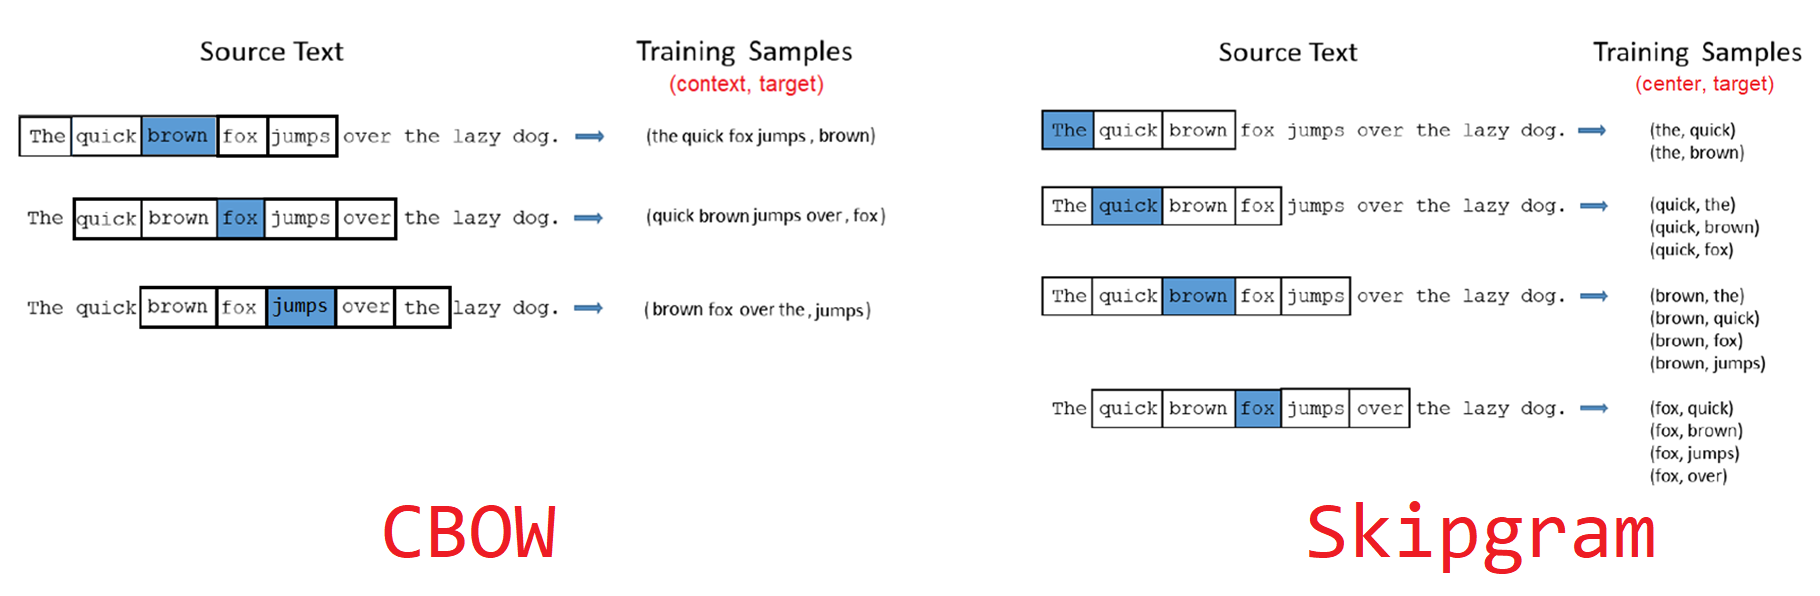
\includegraphics[width=\textwidth]{cbow_sgns2}
    \end{frame}

    \begin{frame}{Word2vec hyperparameters}
        \begin{itemize}
            \item corpus size / source / type
            \item text preprocessing
            \item model type
            \item context window (size of the window)
            \item vector dimensions
        \end{itemize}
    \end{frame}

    \begin{frame}{Semantic relations between words}
        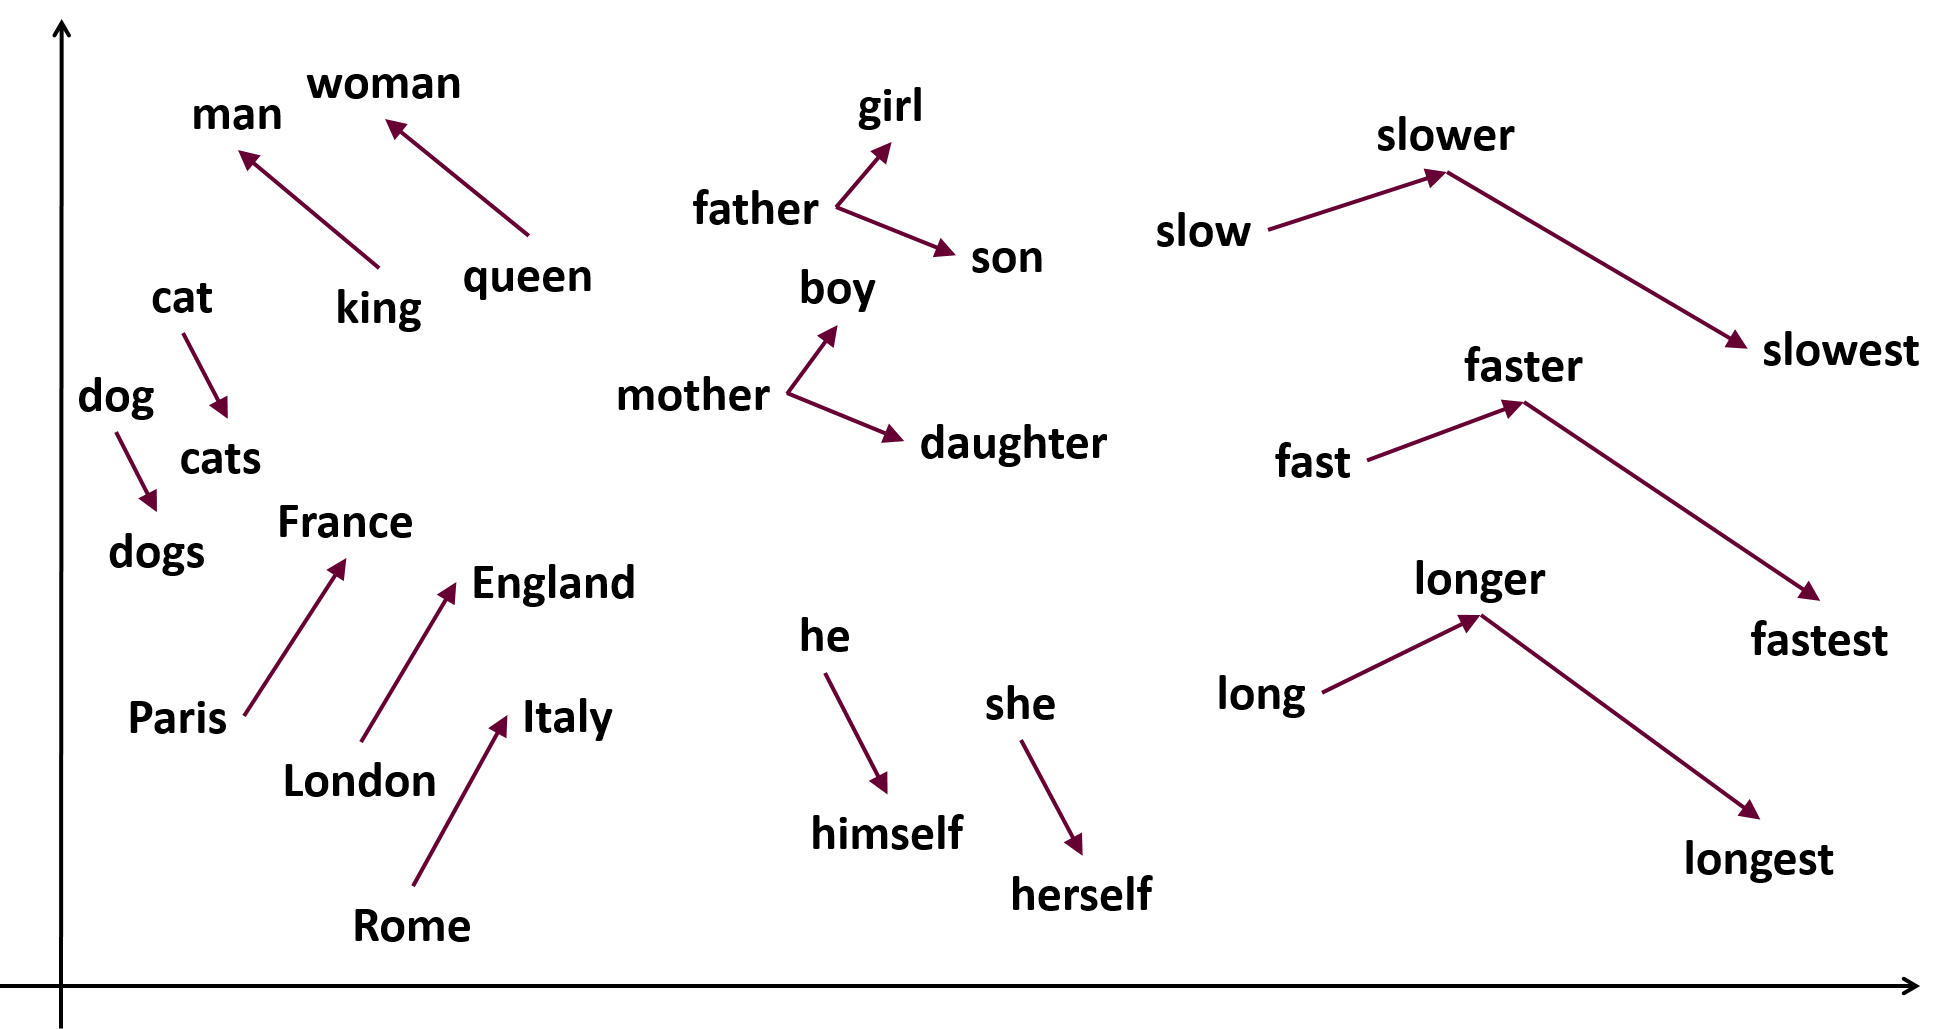
\includegraphics[width=\textwidth]{wvsemantic}
    \end{frame}

    \begin{frame}{Semantic relations between words}
        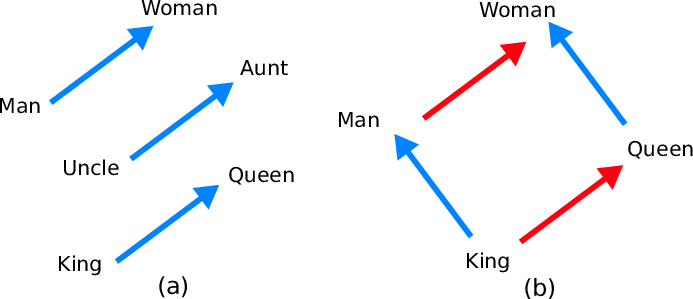
\includegraphics[width=\textwidth]{wvking}
    \end{frame}



    \begin{frame}{Trained WV for Russian}
        \begin{itemize}
            \item Rusvectores \url{https://rusvectores.org/ru/models/}
            \item Navec (from Natasha project) \url{https://github.com/natasha/navec}
            \item Deeppavlov \url{http://docs.deeppavlov.ai/en/master/features/pretrained_vectors.html}
            \item and many many others
        \end{itemize}
    \end{frame}


    \begin{frame}{WE in social science research}
        \begin{itemize}
            \item Train WE on some corpus of interest
            \item Select some words/sets of words corresponding to some concepts from your research
            \item Look at the words relations, change of this relation in time
        \end{itemize}
    \end{frame}


%    \begin{frame}{Examples of WE for social science research}
%
%    \end{frame}
%
%
%    \begin{frame}{Examples of WE for social science research}
%
%    \end{frame}

    \begin{frame}
        \frametitle{Examples of WE for social science research}
        \includegraphics<1>[width=\textwidth]{semantic_change}
        \includegraphics<2>[width=\textwidth]{hamilton-drift}
        % добавить картинки из Гамильтона

        \only<1>{Hamilton W. L., Leskovec J., Jurafsky D. Diachronic Word Embeddings Reveal Statistical Laws of Semantic Change //Proceedings of the 54th Annual Meeting of the Association for Computational Linguistics (Volume 1: Long Papers). – 2016. – С. 1489-1501.
        }
        \only<2>{Hamilton W. L. et al. Inducing domain-specific sentiment lexicons from unlabeled corpora //Proceedings of the Conference on Empirical Methods in Natural Language Processing. Conference on Empirical Methods in Natural Language Processing. – NIH Public Access, 2016. – Т. 2016. – С. 595.}
    \end{frame}


    \begin{frame}{Senetences and documents embeddings}
        \begin{itemize}
            \item Often in the task of text analysis, the necessary embeddings are not words in documents, but the documents themselves or their parts
            \item The easiest way to get it is a weighted sum word embeddings (e.g. with tf-idf as weights)
            This approach shows good results and is often used
            in practice, but there are more interesting methods
            \item If there is a good way to find sentence embedding, vector
            document can again be obtained by averaging over
            sentences
            \item Quality is assessed by the task metric (external criterion) or,
            for example, searching for the quality of labeled analogues (internal)
            \item many other methods, for example, doc2vec
        \end{itemize}
    \end{frame}
\end{document}





